%!TeX spellcheck = en-US
\documentclass{article}
\usepackage{bookmark}
\usepackage{color}
\usepackage{amsmath}
\usepackage{hyperref}
\usepackage{listings}
\usepackage{xcolor}
\usepackage{url}
\usepackage{indentfirst}
\usepackage{graphicx}
\usepackage{amsfonts}
\usepackage{hyperref}
\usepackage[top=2cm, bottom=2cm, left=2cm, right=2cm]{geometry}  
\usepackage{algorithm}  
\usepackage{algorithmicx}  
\usepackage{algpseudocode} 
\usepackage{forest}
\newcommand{\bigO}{\mathcal{O}}
\usepackage{listings}
 
\renewcommand{\algorithmicrequire}{\textbf{Input:}}  
\renewcommand{\algorithmicensure}{\textbf{Output:}}  

\begin{document}
\noindent

%========================================================================
\noindent\framebox[\linewidth]{\shortstack[c]{
\Large{\textbf{VE 477 Homework8}}\vspace{1mm}\\
Wang Yichao, ID: 517370910011}}

\begin{itemize}

\item \textbf{Exercise 1.}

This problem comes from a paper Fast Multipoint Evaluation On n
Arbitrary Points and we need to learn FastEval algorithm. 

\url{http://www.cecm.sfu.ca/CAG/theses/justine.pdf}

Part 1:

1. The split is similar to merge sort. 
\begin{center}
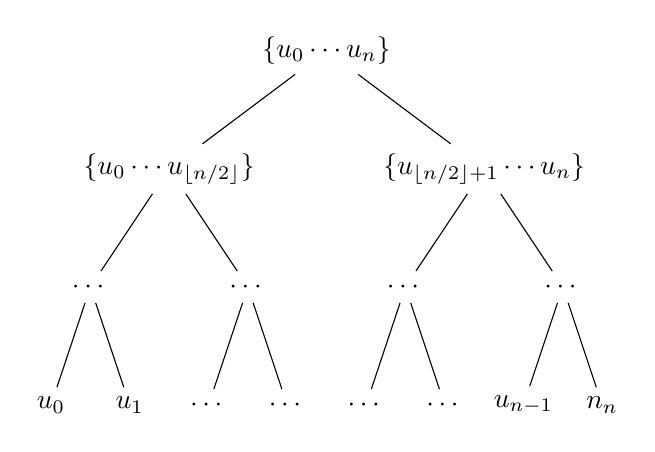
\begin{tikzpicture} 
\tikzstyle{level 1}=[sibling distance=40mm]
\tikzstyle{level 2}=[sibling distance=20mm]
\tikzstyle{level 3}=[sibling distance=10mm]
\node {$\{u_0 \cdots u_n\}$}
child {node {$\{u_0 \cdots u_{\lfloor n/2 \rfloor }\}$}
	child {node { $\cdots$}
		child {node {$u_0$}}
		child {node {$u_1$}}
	}
	child {node { $\cdots$}
		child {node { $\cdots$}}
		child {node { $\cdots$}}
	}
}
child {node {$\{ u_{\lfloor n/2 \rfloor+1} \cdots u_n\}$}
	child {node { $\cdots$}
		child {node { $\cdots$}}
		child {node { $\cdots$}}
	}
	child {node { $\cdots$}
		child {node { $u_{n-1}$}}
		child {node { $n_{n}$}}
	}
};
\end{tikzpicture}
\end{center}

2. It is obvious that when subscript is 0 $M_{0, j}=m_{j+0}= m_{j}$.

When subscript is greater than 0, 
$\begin{aligned}
M_{i+1, j} &=\prod_{l=0}^{2 \cdot 2^{i}-1} m_{j \cdot 2^{i}+l} \\
&=\prod_{l=0}^{2^{i}-1} m_{j \cdot 2^{i}+l} \cdot \prod_{l=2^{i}}^{2 \cdot 2^{i}-1} m_{j \cdot 2^{i}+l} \\
&=\prod_{l=0}^{2^{i}-1} m_{j \cdot 2^{i}+l} \cdot \prod_{l=0}^{2^{i}-1} m_{j \cdot 2^{i}+2^{i}+l} \\
&=M_{i, 2 j} \cdot M_{i, 2 j+1}
\end{aligned}$

3. Since in tree the children of i is $2i$ and $2i+1$, we can learn that parent is the product of its two children.

4. (a) The basic idea is using the product property and build this tree from bottom to the top.

\begin{algorithm}[H]  
    \caption{Build Tree}  
    \begin{algorithmic}[1]  
        \Require an integer $n = 2^k$, $u_0, \cdots, u_{n-1}$ in commutative Ring R
        \Ensure The polynomials $M_{i, j}$ for $0 \leq i \leq k$ and $0 \leq j<2^{k-i}$

        \For {$j = 0, \cdots, n-1$}
            \State $M_{i,j} = x - u_i$
        \EndFor
        \For {$i = 0, \cdots, k$}
        	\For {$j = 0, \cdots, 2^{k-i}-1$}
            	\State $M_{i,j} = M_{i-1,2j}\times M_{i-1,2j+1}$
        	\EndFor
        \EndFor

    \end{algorithmic}  
\end{algorithm}

(b) Use divide and conquer.

\begin{algorithm}[H]  
    \caption{$Recursive$}  
    \begin{algorithmic}[1]  
        \Require an integer $n = 2^k$, $f \in R[x]$ of degree less than $n$, $u_0, \cdots, u_{n-1}$ in commutative Ring R, and polynomials $M_{i, j}$
        \Ensure $f\left(u_{0}\right), \ldots, f\left(u_{n-1}\right)$
        \If {$n == 1$}
        	\State return f
        \EndIf
        \State $r_0 \equiv f \mod M_{k_1, 0}$
		\State $r_1 \equiv f \mod M_{k_1, 1}$

		\State $r_{0}\left(u_{0}\right), \ldots, r_{0}\left(u_{n / 2-1}\right) =Recursive(n/2, r_0, subtree\ rooted\ at\ M_{k_1, 0}$)
		\State $r_{1}\left(u_{n / 2}\right), \ldots, r_{1}\left(u_{n-1}\right) =Recursive(n/2, r_1, subtree\ rooted\ at\ M_{k_1, 1}$)

        \State \Return $r_{0}\left(u_{0}\right), \ldots, r_{0}\left(u_{n / 2-1}\right), r_{1}\left(u_{n / 2}\right), \ldots, r_{1}\left(u_{n-1}\right)$

    \end{algorithmic}  
\end{algorithm}

5. (a) We have already proved that parent is the product of its two children. For $k = 0$, it is trivial since it is constant function and it will return f. Now we assume this is true for k and we need to prove that it is also true for $k+1$. We now do division with remainder. In the $Recursive$ algorithm, for $0\leq i < n/2$, we have $f(u_i) \equiv q_{0}\left(u_{i}\right) \cdot M_{k-1,0}\left(u_{i}\right)+r_{0}\left(u_{i}\right) \equiv r_{0}\left(u_{i}\right)$. For $n/2 \leq i < n$, we have $f(u_i) \equiv q_{1}\left(u_{i}\right) \cdot M_{k-1,1}\left(u_{i}\right)+r_{1}\left(u_{i}\right) \equiv r_{1}\left(u_{i}\right)$. Qed.

(b) For building the tree, the time complexity would be $\frac{n}{2} \mathrm{M}(2)+\frac{n}{4} \mathrm{M}(4)+\cdots+4 \mathrm{M}\left(\frac{n}{4}\right)+2 \mathrm{M}\left(\frac{n}{2}\right) = n\log n^2= \log n M(n)$.

For $Recursive$ algorithm, we have $T (n) = 2T (n/2) + 2D(n)$, where $D(n)$ is  $\bigO(n\log n)$. Using master theorem, we can get the complexity of $T(n) = \bigO(n\log n^2) = \bigO(M(n)\log n)$.

Part 2.

1. 
Strict definition:
Reference: \url{https://www.math.usm.edu/lambers/mat772/fall10/lecture5.pdf}

Readable one:
Reference: \url{https://brilliant.org/wiki/lagrange-interpolation/}

Briefly, if we are given n discrete points, Lagrange interpolation can be used to determine a polynomial that cross these n points, which is fitting.

2. Since $(uv)' = u'v + uv'$, we can get $$m' = m\times \sum_{j=0}^{n-1} \frac{(x-u_j)'}{x-u_j} = m\times \sum_{j=0}^{n-1}\frac{1}{x-u_j}$$(where, $x\not \in \{u_0, \cdots, u_{n-1} \}$). 

When $x=u_i$, only the ith term remains, since for other terms in the summation, m will be 0. Thus $m^{\prime}\left(u_{i}\right)=1 / s_{i}$.

3. Use the similar divide and conquer algorithm as in part 1 question 4.
\begin{algorithm}[H]  
    \caption{$Divide$}  
    \begin{algorithmic}[1]  
        \Require $u_0, \cdots, u_{n-1}$, P
        \Ensure the interpolation of P at the points $u_0, \cdots, u_{n-1}$
        \If {$degree == 1$}
        	\State \Return P
        \EndIf
        \State $r_0 \equiv P \mod M_{k_1, 0}$
		\State $r_1 \equiv P \mod M_{k_1, 1}$
        \State $r_0(u_0), \cdots, P(u_n/2) = Divide(n/2, r_0, subtree\ rooted\ at\ M_{k_1, 0})$
        \State $r_1(u_0), \cdots, P(u_n/2) = Divide(n/2, r_1, subtree\ rooted\ at\ M_{k_1, 1})$
        
        \State \Return $r_{0}\left(u_{0}\right), \ldots, r_{0}\left(u_{n / 2-1}\right), r_{1}\left(u_{n / 2}\right), \ldots, r_{1}\left(u_{n-1}\right)$

    \end{algorithmic}  
\end{algorithm}

4. (a) Optional and not interested.

(b) Similar to part 1, to build up the tree, we need $n\log n^2= \log n M(n)$.

(c) Similar to part 1, for the recursion, we have $T (n) = 2T (n/2) + 2D(n)$, where $D(n)$ is  $\bigO(n\log n)$. Using master theorem, we can get the complexity of $T(n) = \bigO(n\log n^2) = \bigO(M(n)\log n)$. SO it can be solved within $\bigO(M(n)\log n)$ operations.

5. I do not think so, since it will require $\bigO(n^2)$ polynomial space complexity, which is really costly when more points are chosen for fitting. Space is more expensive than time. However, we can do pre-calculation when the size is small to save time. 

\item \textbf{Exercise 2.}

1. Life will be better if we focus on theory instead of coding.

Since $xyxy = yxyx$, assume $xy = m$, we will get $mm = ymx = x^{-1}mmx$, that is $xmm = mmx$ for any x and m, we denote this equation as lemma.

Next we prove that $(xyx^{-1}y^{-1})^4 = e$. We rewrite it as 

$(xyx^{-1}y^{-1})^2 (xyx^{-1})y^{-1} xyx^{-1}y^{-1} \\= (xyx^{-1}) (xyx^{-1}y^{-1})^2 y^{-1} xyx^{-1}y^{-1}$ (by taking $xyx^{-1}y^{-1}$ as m in lemma) \\$= xy^2x^{-1}y^{-1}xyx^{-1}(y^{-1})^2xyx^{-1}y^{-1}$ (then we take advantage of two squares in this line) \\$= y^2xx^{-1}y^{-1}xyx^{-1}(y^{-1})^2xyx^{-1}y^{-1}$ \\$= yxyx^{-1}(y^{-1})^{2} x y x^{-1} y^{-1}$ \\$ = yxyx^{-1}x(y^{-1})^{2} y x^{-1} y^{-1}$\\$ = e$.

Finally since $(xyx^{-1}y^{-1})^4 = e$, we can get $(xyx^{-1}y^{-1})^2 = e$, then $(xyx^{-1}y^{-1}) = e$, which means $xy = yx$. Qed.

2. Talk is cheap, show me the code. I reckon that it is impossible to calculate this question by hand. I am really curious how can our smart ATIJ solve this problem by hand.

From what $S_2$ says, there are at least two ways to divide the xy. So this problem is about factorization. From what $S_1$ says, we can learn that there is no way to divide $x+y$ into to numbers such that the multiple of them has only one way of factorization into two integer greater than 1. Now we assume $x + y = m$ and $x\times y = n$. Then according to our reasoning. $n = p_1\times p_2\times q$ and $m = prime + composite$ or $m = composite + composite$. There is only one way for n to be divided.

I use brute force to solve this problem in python. the runtime is OK for small input like this, but further \textbf{optimization} is required for larger input!!!

type \textbf{./run.sh} in terminal, the answer will be redirected to stdout.txt
the answer is in the last line, all the lines above are the key processes

\item \textbf{Exercise 3.}

Swype keyboard is a special way of typing English letters(also support other languages). Instead of pressing each letter once a time, you draw fold lines between each letter you want to type in and you do not need to move your fingers off the screen. There is an advanced algorithm to solve the accuracy problem since the path of your finger is hard to interpret directly. This Swype service is not available after 2018. My roommate is lucky to have tried this technology before on his phone.

Reference: \url{https://www.youtube.com/watch?v=SJ-RAefCG_c}

\item \textbf{Exercise 4.}

I have completed the course survey. 

\end{itemize}

%========================================================================
\end{document}
















